% Figure 1 (V7.1): edge-to-cloud data path, trust boundaries and attacker positions.
% Drawn at final size: included at scale 1 in the MDPI full width (18.47 cm); box titles 9 pt, all other text 8 pt;
% notation as in Section 4 (origin key k_o and signature sigma_o, relay key k_w and signature sigma_w).
% All line breaks are explicit (no automatic breaking), so no word is hyphenated inside a box.
\documentclass[tikz,border=2pt]{standalone}
\usepackage[T1]{fontenc}
\usepackage{mathpazo}
\usetikzlibrary{positioning,arrows.meta,fit,backgrounds,calc}
\definecolor{ot}{HTML}{EAF2E3}\definecolor{edge}{HTML}{E4ECF6}\definecolor{conduit}{HTML}{F7F0E1}
\definecolor{cloud}{HTML}{ECE8F5}\definecolor{plat}{HTML}{F1F1F1}\definecolor{att}{HTML}{B3261E}
\definecolor{acc}{HTML}{2F5D8A}
\tikzset{
 box/.style={draw=black!70,rounded corners=2pt,fill=white,align=center,font=\footnotesize,inner sep=2.5pt},
 zone/.style={draw=black!45,dashed,rounded corners=5pt,inner xsep=4pt,inner ysep=5pt},
 flow/.style={-{Latex[length=2mm]},thick,black!75},
 ctl/.style={-{Latex[length=1.8mm]},black!60,densely dashed},
 ap/.style={circle,draw=att,thick,fill=white,text=att,font=\footnotesize\bfseries,inner sep=0.3pt,minimum size=6.4mm},
 zl/.style={font=\footnotesize\bfseries,text=black!70,anchor=south west,inner sep=1pt}
}
\newcommand{\T}[1]{{\small #1}}
\begin{document}
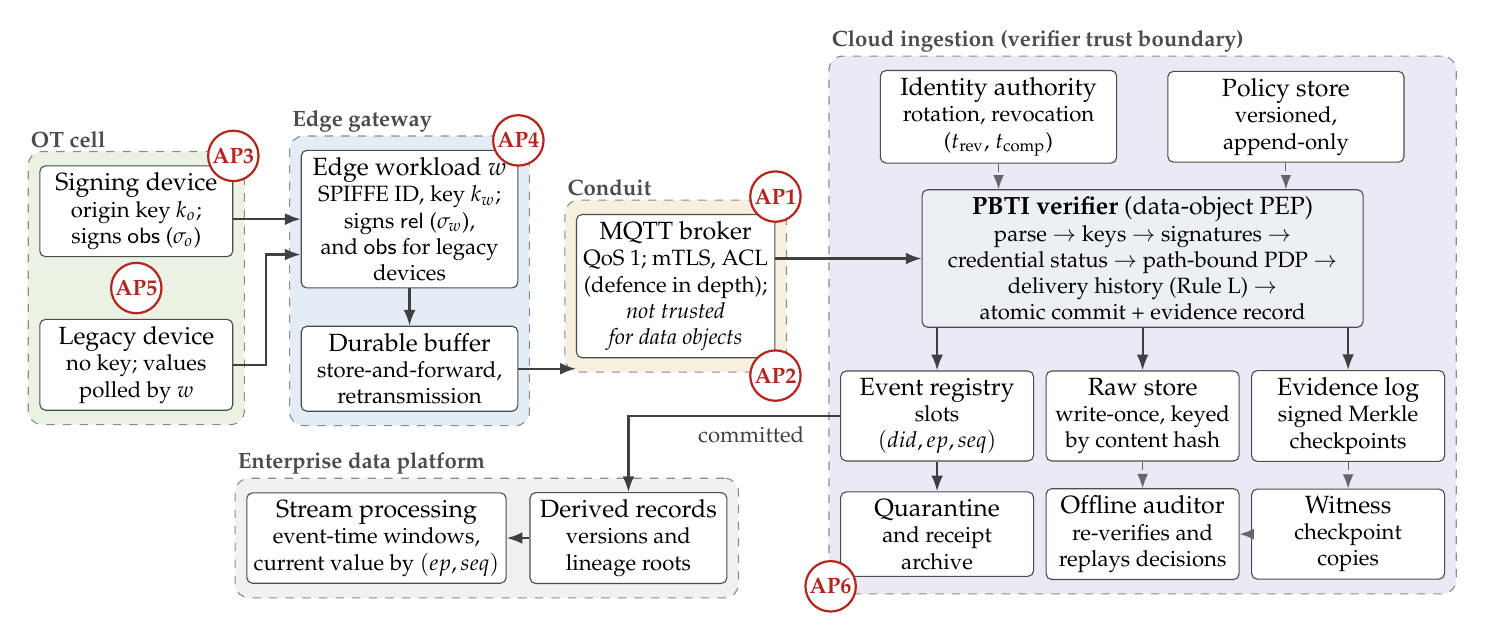
\begin{tikzpicture}
% ---------------------------------------------------------------- OT cell
\node[box,minimum width=24.5mm] (dev) at (1.35,1.55) {\T{Signing device}\\origin key $k_o$;\\signs \textsf{obs} ($\sigma_o$)};
\node[box,minimum width=24.5mm] (leg) at (1.35,-0.4) {\T{Legacy device}\\no key; values\\polled by $w$};
% ---------------------------------------------------------------- edge gateway
\node[box,minimum width=27.5mm] (wl) at (4.82,1.45) {\T{Edge workload $w$}\\SPIFFE ID, key $k_w$;\\signs \textsf{rel} ($\sigma_w$),\\and \textsf{obs} for legacy\\devices};
\node[box,minimum width=27.5mm] (buf) at (4.82,-0.45) {\T{Durable buffer}\\store-and-forward,\\retransmission};
% ---------------------------------------------------------------- conduit
\node[box,minimum width=25mm] (brk) at (8.2,0.6) {\T{MQTT broker}\\QoS 1; mTLS, ACL\\(defence in depth);\\\emph{not trusted}\\\emph{for data objects}};
% ---------------------------------------------------------------- cloud ingestion
\node[box,minimum width=56mm,fill=acc!9] (ver) at (14.13,0.95)
 {\T{\textbf{PBTI verifier} (data-object PEP)}\\
  parse $\rightarrow$ keys $\rightarrow$ signatures $\rightarrow$\\
  credential status $\rightarrow$ path-bound PDP $\rightarrow$\\
  delivery history (Rule L) $\rightarrow$\\
  atomic commit + evidence record};
\node[box,minimum width=30mm] (ca) at (12.3,2.75) {\T{Identity authority}\\rotation, revocation\\($t_\mathrm{rev}$, $t_\mathrm{comp}$)};
\node[box,minimum width=30mm] (pdp) at (15.95,2.75) {\T{Policy store}\\versioned,\\append-only};
\node[box,minimum width=24.5mm] (reg) at (11.52,-1.05) {\T{Event registry}\\slots\\$(did,ep,seq)$};
\node[box,minimum width=24.5mm] (raw) at (14.13,-1.05) {\T{Raw store}\\write-once, keyed\\by content hash};
\node[box,minimum width=24.5mm] (ev) at (16.74,-1.05) {\T{Evidence log}\\signed Merkle\\checkpoints};
\node[box,minimum width=24.5mm] (q) at (11.52,-2.55) {\T{Quarantine}\\and receipt\\archive};
\node[box,minimum width=24.5mm] (aud) at (14.13,-2.55) {\T{Offline auditor}\\re-verifies and\\replays decisions};
\node[box,minimum width=24.5mm] (wit) at (16.74,-2.55) {\T{Witness}\\checkpoint\\copies};
% ---------------------------------------------------------------- enterprise data platform
\node[box,minimum width=29mm] (sp) at (4.4,-2.6) {\T{Stream processing}\\event-time windows,\\current value by $(ep,seq)$};
\node[box,minimum width=25mm] (der) at (7.6,-2.6) {\T{Derived records}\\versions and\\lineage roots};
% ---------------------------------------------------------------- zones
\begin{scope}[on background layer]
\node[zone,fill=ot,fit=(dev)(leg)] (zot) {};
\node[zone,fill=edge,fit=(wl)(buf)] (zedge) {};
\node[zone,fill=conduit,fit=(brk)] (zcon) {};
\node[zone,fill=cloud,fit=(ver)(ca)(pdp)(reg)(raw)(ev)(q)(aud)(wit)] (zcl) {};
\node[zone,fill=plat,fit=(sp)(der)] (zpl) {};
\end{scope}
\node[zl] at (zot.north west) {OT cell};
\node[zl] at (zedge.north west) {Edge gateway};
\node[zl] at (zcon.north west) {Conduit};
\node[zl] at (zcl.north west) {Cloud ingestion (verifier trust boundary)};
\node[zl] at (zpl.north west) {Enterprise data platform};
% ---------------------------------------------------------------- flows
\draw[flow] (dev.east|-wl.west) -- (wl.west);
\draw[flow] (leg.east) -- ++(0.42,0) |- ($(wl.west)+(0,-0.45)$);
\draw[flow] (wl) -- (buf);
\draw[flow] (buf.east) -- (brk.west|-buf.east);
\draw[flow] (brk.east|-ver.west) -- (ver.west);
\draw[ctl] (ca) -- (ca|-ver.north);
\draw[ctl] (pdp) -- (pdp|-ver.north);
\draw[flow] (ver.south-|reg) -- (reg);
\draw[flow] (ver.south-|raw) -- (raw);
\draw[flow] (ver.south-|ev) -- (ev);
\draw[flow] (reg) -- (q);
\draw[ctl] (ev) -- (wit);
\draw[ctl] (raw) -- (aud);
\draw[ctl] (wit) -- (aud);
\draw[flow] (reg.west) -- node[below,font=\footnotesize,pos=0.42]{committed} (reg.west-|der.north) -- (der.north);
\draw[flow] (der) -- (sp);
% ---------------------------------------------------------------- attacker positions (Table 2)
\node[ap] at ($(brk.north east)+(0,0.22)$) {AP1};
\node[ap] at ($(brk.south east)+(0,-0.22)$) {AP2};
\node[ap] at ($(dev.north east)+(0,0.12)$) {AP3};
\node[ap] at ($(wl.north east)+(0,0.12)$) {AP4};
\node[ap] at ($(dev.south)!0.5!(leg.north)$) {AP5};
\node[ap] at ($(q.south west)+(-0.12,-0.12)$) {AP6};
\end{tikzpicture}
\end{document}
